%%%%%%%%%%%%%%% Start of Title Page %%%%%%%%%%%
\begin{titlepage}
    \begin{center}
        \textit{Heaven's Light is Our Guide}
        \\[0.5cm]
        \textbf{\Large Rajshahi University of Engineering \& Technology}
        \\[0.3cm]
        \textbf{\large Department of Electronics \& Telecommunication Engineering}
        \\[0.2cm]
        \begin{figure}[!htbp]
            \centering
            
\includegraphics[scale=0.3]{src/logo_ruet}
            \label{fig:RUET logo}
        \end{figure}
        \textbf{\Large ETE 1212: Sessional Based on ETE 1211 }
        \\[0.5cm]
        \myrule[1pt][5pt]

        %%%%%%%%%%%%%%%%%%%%%%%%%%%%%%%%%%%%%%%%%%%%%%%
        %%%%%%%%%%%%%%% STUDENT'S INFO %%%%%%%%%%%%%%%%
        %%%%%%%%%%%%%%%%%%%%%%%%%%%%%%%%%%%%%%%%%%%%%%%

        \textbf{\Large  Experiment No. 03}
        \\[.25cm]
        \textbf{\large Experimental Study of diode series connection and diode parallel connection}
        \\
        \myrule[1pt][5pt]
        \begin{minipage}{0.4\textwidth}
            \vspace{0.5cm}
            \begin{flushleft}
                \emph{\textbf{\large Submitted by:}}
                \\
                Shahoriar Rahman \\
                Roll: 2104001 \\
                Session: 2021-22
            \end{flushleft}
        \end{minipage}
        ~
        \begin{minipage}{0.4\textwidth}
            \vspace{0.5cm}
            \begin{flushright}
                \emph{\textbf{\large Submitted to:}}
                \\
                Hasan Sarker
                \\
                Lecturer
                \\
                Dept. of ETE, RUET
                \\
            \end{flushright}
        \end{minipage}\\[0.7cm]
        \makeatother

        \textbf{Date of Experiment : 23/07/2023}\\
        \textbf{Date of Submission : 30/07/2023}\\[1cm]

        %************** End of Student's Info *********


        \vfill
        %%%%%%%%%%%%%%% TEACHER SECTION %%%%%%%%%%%%%%%
        \hrulefill
        \vspace{-5mm}
        \begin{multicols}{3}
            \begin{itemize} [labelindent=3em,labelsep=0.5cm,leftmargin=*,noitemsep]
                \item[] \textbf{\underline{Report}}
                \item[$\square$] Excellent
                \item[$\square$] Very Good
                \item[$\square$] Good
                \item[$\square$] Average
                \item[$\square$] Poor
            \end{itemize}
            \columnbreak
            \textbf{(Teacher's Section)}
            \\[1.5cm]
            --------------------------------
            \\
            Signature
            \columnbreak
            \begin{itemize}
                [labelindent=6em,labelsep=0.5cm,leftmargin=*,noitemsep]
                \item[] \textbf{\underline{Viva}}
                \item[$\square$] Excellent
                \item[$\square$] Very Good
                \item[$\square$] Good
                \item[$\square$] Average
                \item[$\square$] Poor
            \end{itemize}
        \end{multicols}
    \end{center}
\end{titlepage}

%************** End of Teacher Section ********
%************** End of Title Page *************


%%%%%%%%%%%%%%% Exp. Positioning %%%%%%%%%%%%%%
\titleformat{\chapter}[display]
{\normalfont\large\bfseries}{Experiment Name: 0\thechapter}{0pt}{\large}

\titlespacing*{\chapter}{0pt}{-15pt}{10pt}
% \addcontentsline{lof}{chapter}{\protect\numberline{ \ref{exp1}}}
% \addcontentsline{lot}{chapter}{\protect\numberline{ \ref{exp1}}}
%************** End of Exp. Positioning *******


%%%%%%%%%%%%%%%%%%%%%%%%%%%%%%%%%%%%%%%%%%%%%%%
%%%%%%%%%%%%%%% Student's Part %%%%%%%%%%%%%%%%
%%%%%%%%%%%%%%% Start of Report %%%%%%%%%%%%%%%
%%%%%%%%%%%%%%%%%%%%%%%%%%%%%%%%%%%%%%%%%%%%%%%


%**********************************************
\chapter{Experiment Name: Experimental Study of diode series connection and diode parallel connection}
\label{exp1}


%**********************************************
\section{Objectives}
The main objectives of this experiment are
\begin{enumerate}
    \item To learn the properties of series connection
    \item To determine the voltage drop for each diode
    \item To understand the phenomenon when a diode is connected reverse biasing in series
\end{enumerate}

\section{Theory}
\begin{enumerate}
    \item Potential difference across every component is different.
    \item The current across every component connected in series remains the same.
\end{enumerate}
A parallel connection is when multiple components are connected side by side, sharing
the same voltage across their terminals but having independent current paths. The total
current flowing into the parallel connection is divided among the components based on their
individual resistance.

\subsection{Forward Bias}
When the external voltage is applied across the P-N junction diode, this is known as forward
bias or biasing. The P-side of the diode is connected to the positive terminal, and the N-
side is fastened to the battery’s negative side in a forward bias setup. The junction barrier
potential is opposite to the applied voltage in this instance.
\begin{figure}[H]
    \centering
    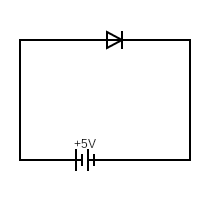
\includegraphics[scale=0.6]{src/exp02/circuit (3).png}
    \caption{Forward Bias of Diode}
\end{figure}
\subsection{Reverse Bias}
Reverse bias refers to the application of an external voltage across a semiconductor diode
such that the positive terminal of the battery is connected to the n-side and the negative
terminal is connected to the p-side of the diode.
\begin{figure}[H]
    \centering
    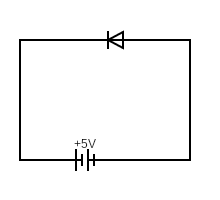
\includegraphics[scale=0.6]{src/exp02/circuit (4).png}
    \caption{Reverse Bias of Diode}
\end{figure}

\section{Required Components}
\begin{enumerate}
    \item P-N Junction Diode (2pcs, in 4007))
    \item Resistors(2 pieces; 100 $\Omega$)
    \item Project Board
    \item Multimeter (2 pieces)
    \item Jumper Cables
    \item Variable DC source (0-15V)
\end{enumerate}

\section{Circuit Diagram}
\begin{figure}[H]
    \centering
    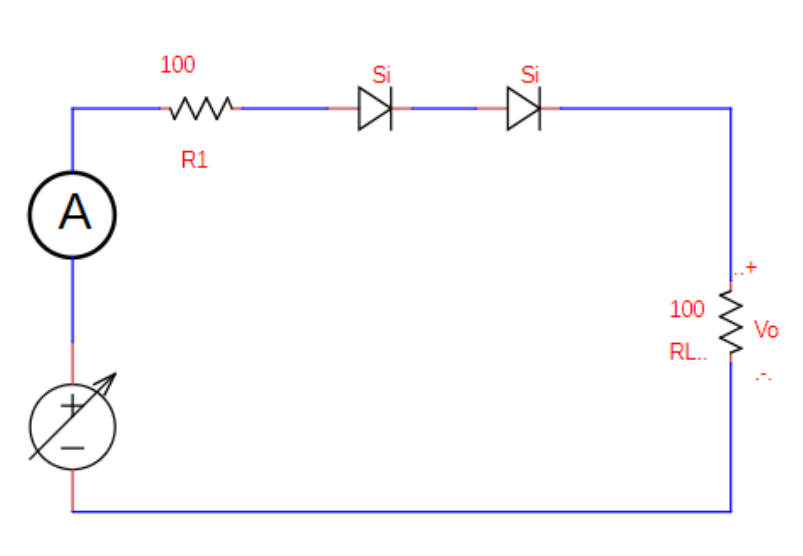
\includegraphics[scale=0.3]{src/exp03/fig1.png}
    \caption{Forward bias series diode circuit connection.}
\end{figure}

\begin{figure}[H]
    \centering
    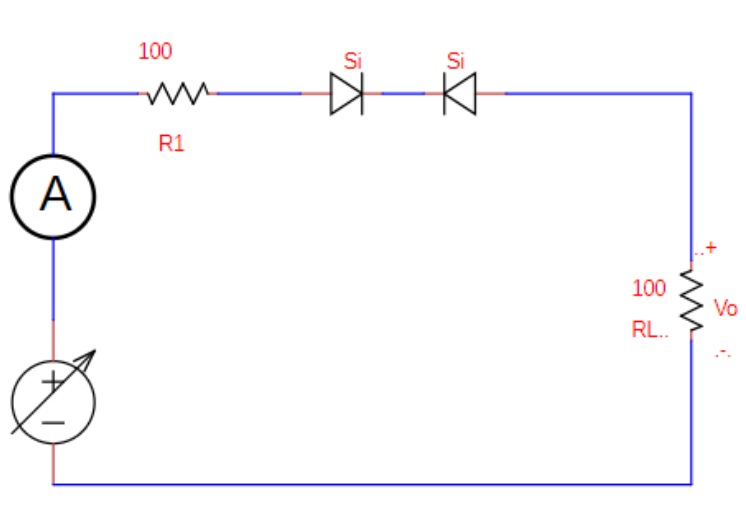
\includegraphics[scale=0.3]{src/exp03/fig2.png}
    \caption{Reverse bias series diode circuit connection.}
\end{figure}

\begin{figure}[H]
    \centering
    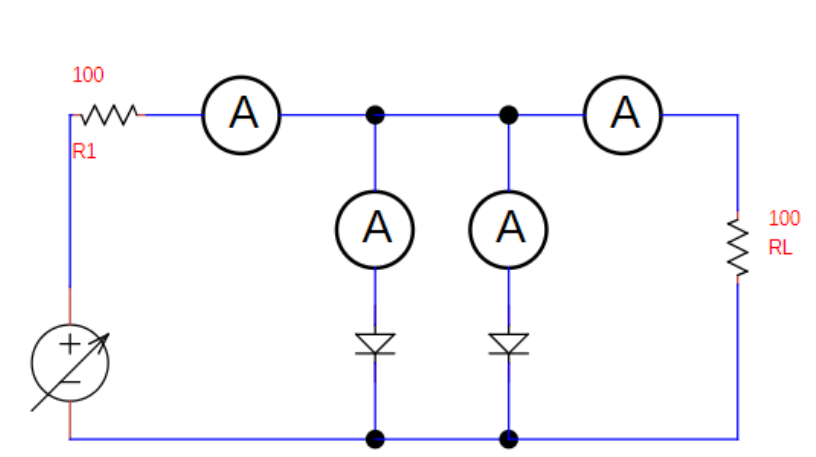
\includegraphics[scale=0.3]{src/exp03/fig3.png}
    \caption{Forward bias parallel diode circuit connection.}
\end{figure}

\begin{figure}[H]
    \centering
    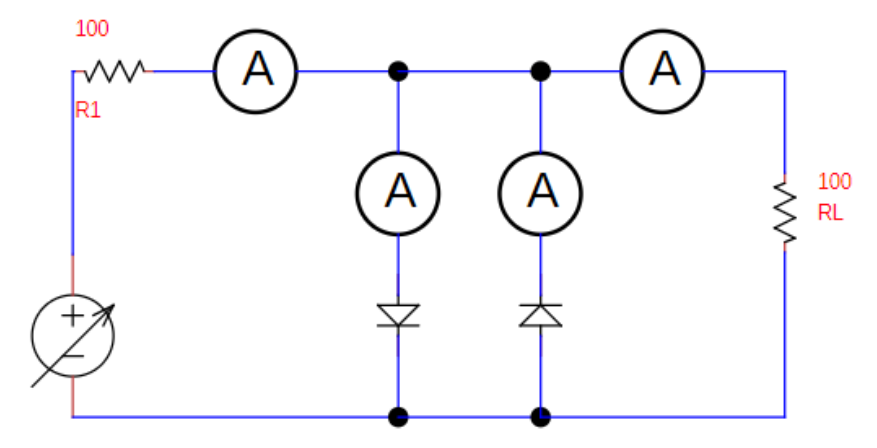
\includegraphics[scale=0.3]{src/exp03/fig4.png}
    \caption{Reverse bias parallel diode circuit connection.}
\end{figure}

\section{Experimental Work}
\subsection{Experimental setup for series diode connection}
\begin{figure}[H]
    \centering
    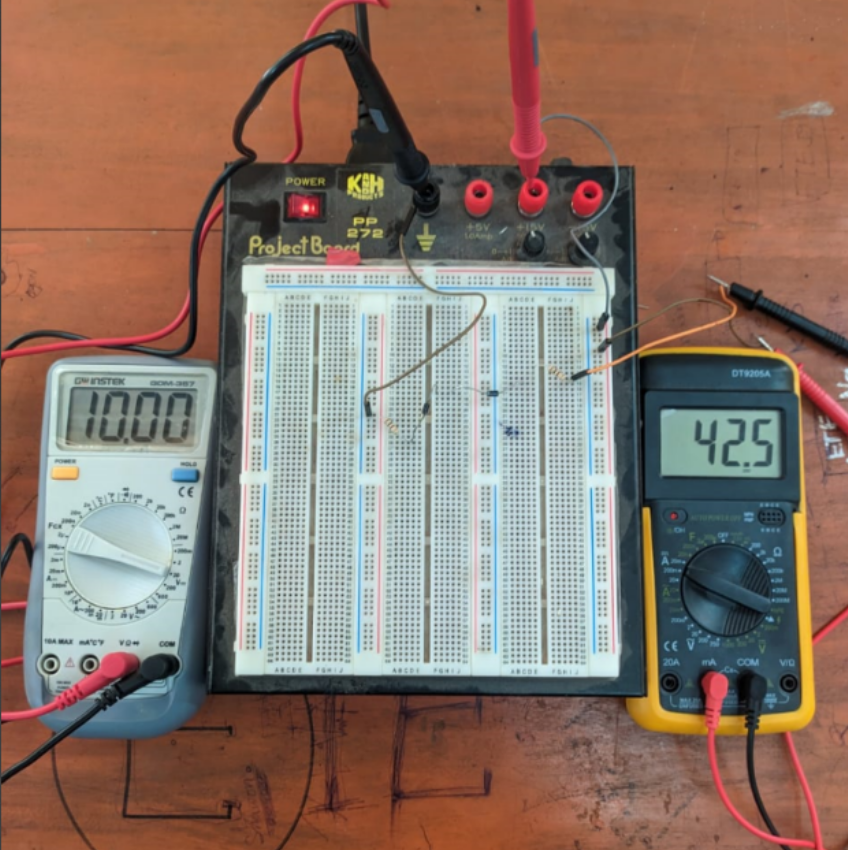
\includegraphics[scale=0.3]{src/exp03/ser1.png}
    \caption{Forward diode series connection.}
\end{figure}
\begin{figure}[H]
    \centering
    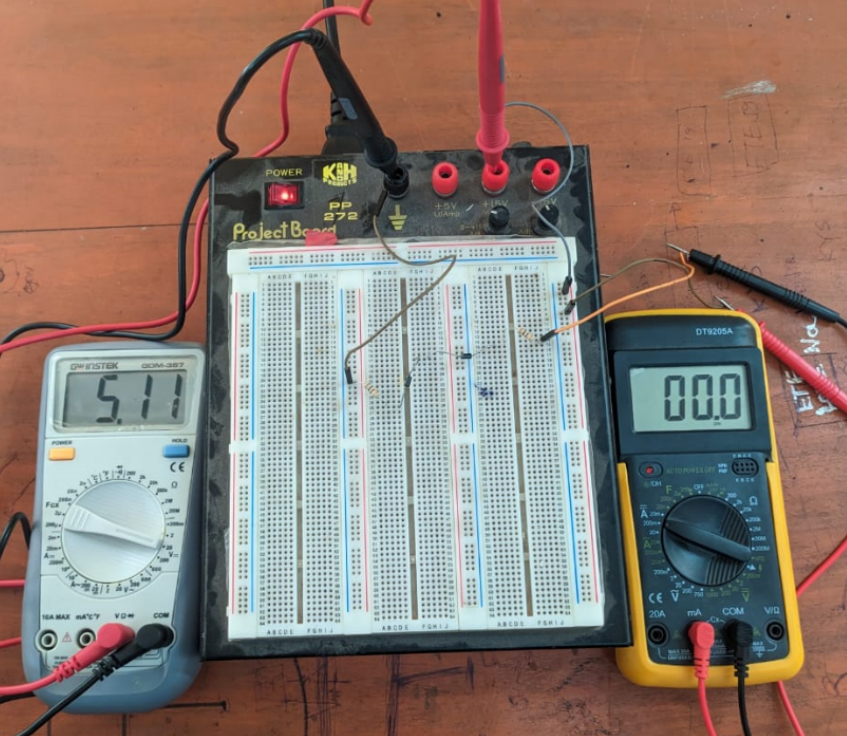
\includegraphics[scale=0.3]{src/exp03/ser2.png}
    \caption{Reverse diode series connection.}
\end{figure}
\subsection{Experimental setup for parallel diode connection}
\begin{figure}[H]
    \centering
    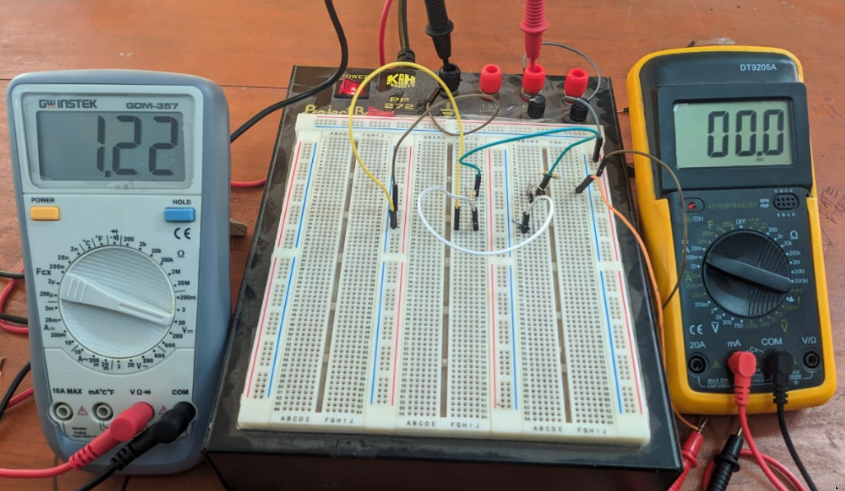
\includegraphics[scale=0.3]{src/exp03/par1.png}
    \caption{Forward diode parallel connection.}
\end{figure}

\begin{figure}[H]
    \centering
    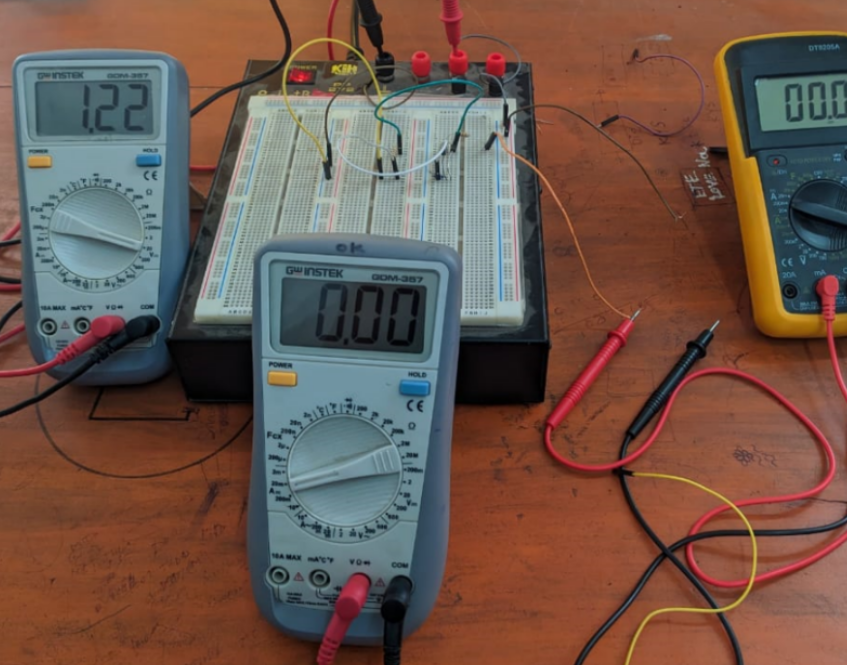
\includegraphics[scale=0.3]{src/exp03/par2.png}
    \caption{Reverse diode parallel connection.}
\end{figure}

\section{Experimental Data}

\begin{table}[hbt!]
    \centering
    \caption{ Forward Bias Series Connection.}
    \label{tab1}


    \begin{tabular}{|l|l|l|l|l|l|l|l|}
        \hline
        S.L & Vin    & I    & VD1   & VD2   & VR1  & VR2  & Error (\%) \\ \hline
        1   & 1.22   & 0    & 0.58  & 0.75  & 0    & 0    & 9.01       \\ \hline
        2   & 5.02   & 16.9 & 0.71  & 0.71  & 1.69 & 1.69 & 4.38       \\ \hline
        3   & 6.01   & 22.7 & 0.72  & 0.74  & 2.26 & 2.26 & 0.5        \\ \hline
        4   & 8.00   & 32.3 & 0.74  & 0.78  & 3.19 & 3.19 & 1.25       \\ \hline
        5   & 10.05  & 42.6 & 0.75  & 0.31  & 4.19 & 4.18 & 6.17       \\ \hline
        6   & -10.01 & 0    & -3.42 & -1.95 & 0    & 0    &            \\ \hline
    \end{tabular}
\end{table}
\begin{table}[hbt!]
    \centering
    \caption{Reverse Bias Series Connection.}
    \label{tab2}
    \begin{tabular}{|l|l|l|l|l|l|l|l|}
        \hline
        S.L & Vin    & I & VD1   & VD2  & VR1 & VR2 & Error (\%) \\ \hline
        1   & 1.25   & 0 & -0.73 & 1.75 & 0   & 0   & 9.01       \\ \hline
        2   & 5.08   & 0 & -0.81 & 3.04 & 0   & 0   & 4.38       \\ \hline
        3   & 5.97   & 0 & -0.78 & 5.66 & 0   & 0   & 0.5        \\ \hline
        4   & 8.00   & 0 & -0.7  & 8.2  & 0   & 0   & 1.25       \\ \hline
        5   & 10.02  & 0 & -0.95 & 9.7  & 0   & 0   & 6.17       \\ \hline
        6   & -10.05 & 0 & -11.3 & 2.79 & 0   & 0   &            \\ \hline
    \end{tabular}
\end{table}

\begin{table}[hbt!]
    \centering
    \caption{Reverse Bias Series Connection.}
    \label{tab2}
    \begin{tabular}{|l|l|l|l|l|l|l|l|l|l|}
        \hline
        S.L & \begin{tabular}[c]{@{}l@{}}Vin\\ (V)\end{tabular} & \begin{tabular}[c]{@{}l@{}}ID1 \\ (mA)\end{tabular} & \begin{tabular}[c]{@{}l@{}}ID2 \\ (mA)\end{tabular} & \begin{tabular}[c]{@{}l@{}}I1 \\ (mA)\end{tabular} & \begin{tabular}[c]{@{}l@{}}I2 \\ (mA)\end{tabular} & \begin{tabular}[c]{@{}l@{}}VR1\\ (V)\end{tabular} & \begin{tabular}[c]{@{}l@{}}VR2\\ (V)\end{tabular} & \begin{tabular}[c]{@{}l@{}}Error (V)\\   (\%)\end{tabular} & \begin{tabular}[c]{@{}l@{}}Error (I)\\   (\%)\end{tabular} \\ \hline
        1   & 3.72                                              & 9.5                                                 & 9.5                                                 & 29.5                                               & 9.8                                                & 2.85                                              & 0.69                                              & 4.84                                                       & 2.73                                                       \\ \hline
        2   & 5.03                                              & 17.7                                                & 17.7                                                & 42.7                                               & 7.6                                                & 4.11                                              & 0.10                                              & 16.3                                                       & 0.70                                                       \\ \hline
        3   & 6.54                                              & 24.9                                                & 24.9                                                & 58.5                                               & 7.6                                                & 5.68                                              & 0.74                                              & 1.83                                                       & 1.88                                                       \\ \hline
        4   & 8.05                                              & 32.3                                                & 32.3                                                & 74.3                                               & 7.7                                                & 7.03                                              & 0.76                                              & 3.23                                                       & 2.7                                                        \\ \hline
        5   & 10                                                & 38.3                                                & 38.3                                                & 96.4                                               & 7.6                                                & 9.03                                              & 0.81                                              & 1.6                                                        & 12.7                                                       \\ \hline
        6   & -10                                               & 0                                                   & 0                                                   & 50.9                                               & 51.2                                               & -4.83                                             & -4.83                                             & 3.4                                                        & 0.6                                                        \\ \hline
    \end{tabular}
\end{table}

\begin{table}[hbt!]
    \centering
    \caption{Reverse Bias parallel Connection.}
    \label{tab2}
    \begin{tabular}{|l|l|l|l|l|l|l|l|l|l|}
        \hline
        S.L & \begin{tabular}[c]{@{}l@{}}Vin\\ (V)\end{tabular} & \begin{tabular}[c]{@{}l@{}}ID1 \\ (mA)\end{tabular} & \begin{tabular}[c]{@{}l@{}}ID2 \\ (mA)\end{tabular} & \begin{tabular}[c]{@{}l@{}}I1 \\ (mA)\end{tabular} & \begin{tabular}[c]{@{}l@{}}I2 \\ (mA)\end{tabular} & \begin{tabular}[c]{@{}l@{}}VR1\\ (V)\end{tabular} & \begin{tabular}[c]{@{}l@{}}VR2\\ (V)\end{tabular} & \begin{tabular}[c]{@{}l@{}}Error (V)\\   (\%)\end{tabular} & \begin{tabular}[c]{@{}l@{}}Error (I)\\   (\%)\end{tabular} \\ \hline
        1   & 3.72                                              & 19                                                  & 0                                                   & 27.7                                               & 8.1                                                & 2.76                                              & 0.75                                              & 5.64                                                       & 2.2                                                        \\ \hline
        2   & 5.03                                              & 32.3                                                & 0                                                   & 39.8                                               & 7.9                                                & 3.96                                              & 0.9                                               & 3.38                                                       & 1                                                          \\ \hline
        3   & 6.54                                              & 47.7                                                & 0                                                   & 56.6                                               & 8.8                                                & 5.49                                              & 0.91                                              & 2.14                                                       & 0.2                                                        \\ \hline
        4   & 8.05                                              & 59.1                                                & 0                                                   & 68.8                                               & 10.5                                               & 6.79                                              & 1.03                                              & 2.86                                                       & 1.16                                                       \\ \hline
        5   & 10                                                & 81.2                                                & 0                                                   & 92.7                                               & 11.9                                               & 8.68                                              & 1.14                                              & 1.8                                                        & 0.43                                                       \\ \hline
        6   & -10                                               & 0                                                   & 82.5                                                & 90.2                                               & 8.41                                               & -8.41                                             & -0.81                                             & 7.8                                                        & 0.79                                                       \\ \hline
    \end{tabular}
\end{table}



\section{Discussion}

The experiment focused on investigating the behavior of diodes in both series and parallel connections under various biasing conditions. When a diode was forward biased in the series configuration, current flowed uniformly throughout the circuit, while the voltage drop across the diode remained consistent at approximately 0.7 volts. Increasing the applied voltage resulted in a proportional rise in current, but the voltage drop across the diode remained constant. Conversely, reverse biasing the diodes in the series connection prevented any current flow.

In the parallel diode connection, each diode operated independently, allowing current flow when forward biased, with a constant voltage drop of around 0.7 volts for each diode. The total current in the parallel connection was the sum of the individual diode currents. However, when one or more diodes were reverse biased, no current flowed through them, while the forward-biased diodes continued to conduct independently.

The parallel diode configuration demonstrated enhanced current-handling capabilities and offered circuit redundancy. This study provides valuable insights into diode behavior under different biasing conditions, which can be applied in electronic circuit design and analysis.
\section{Conclusion}
The experiment's findings indicate that when diodes and loads are connected in series, the current remains constant throughout the circuit. On the other hand, in a parallel configuration, the current is divided among the diodes and loads. Moreover, when one or more diodes are in a state of reverse biasing, no current flows through them. This observation is consistent with the fact that in parallel connections, the reverse diode current is also zero. Furthermore, the experiment revealed that the voltage drop across a diode is approximately in the range of 0.31 to 0.78 volts. These results provide valuable insights into the behavior of diodes in different configurations and biasing conditions, serving as a basis for the design and analysis of electronic circuits.
\newpage

\begin{figure}[H]
    \centering
    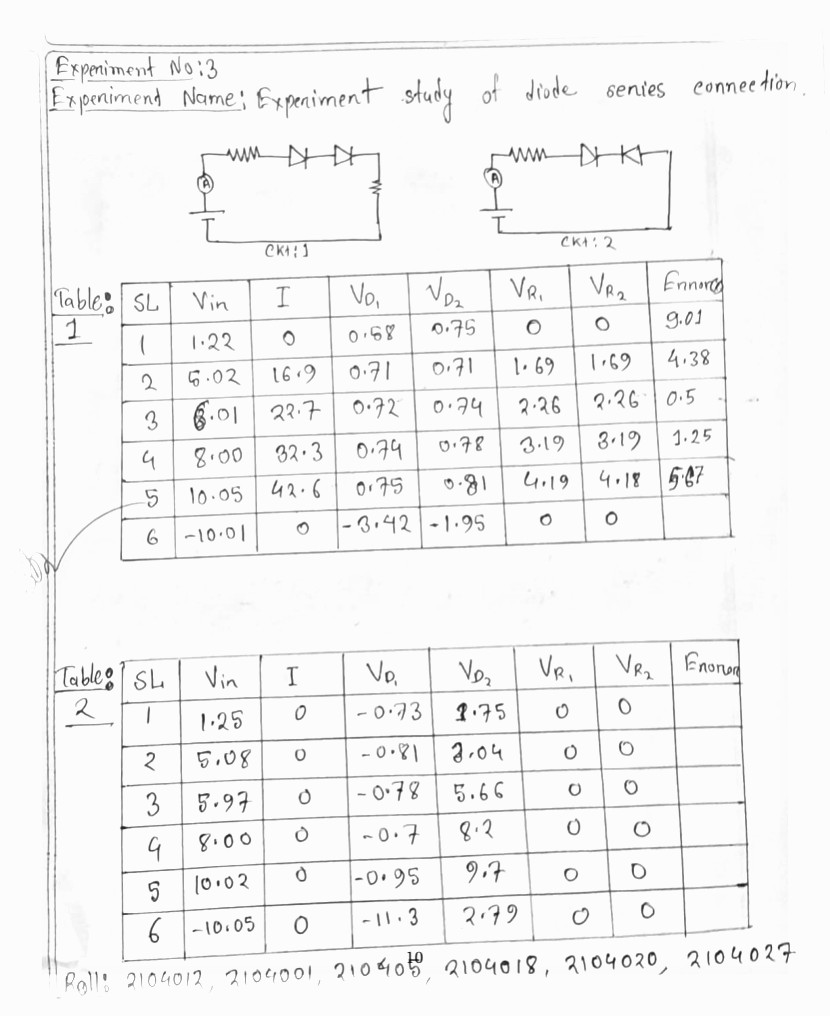
\includegraphics[scale=0.6]{src/exp03/r1.jpg}

    \caption{}
\end{figure}
\newpage

\begin{figure}[H]
    \centering
    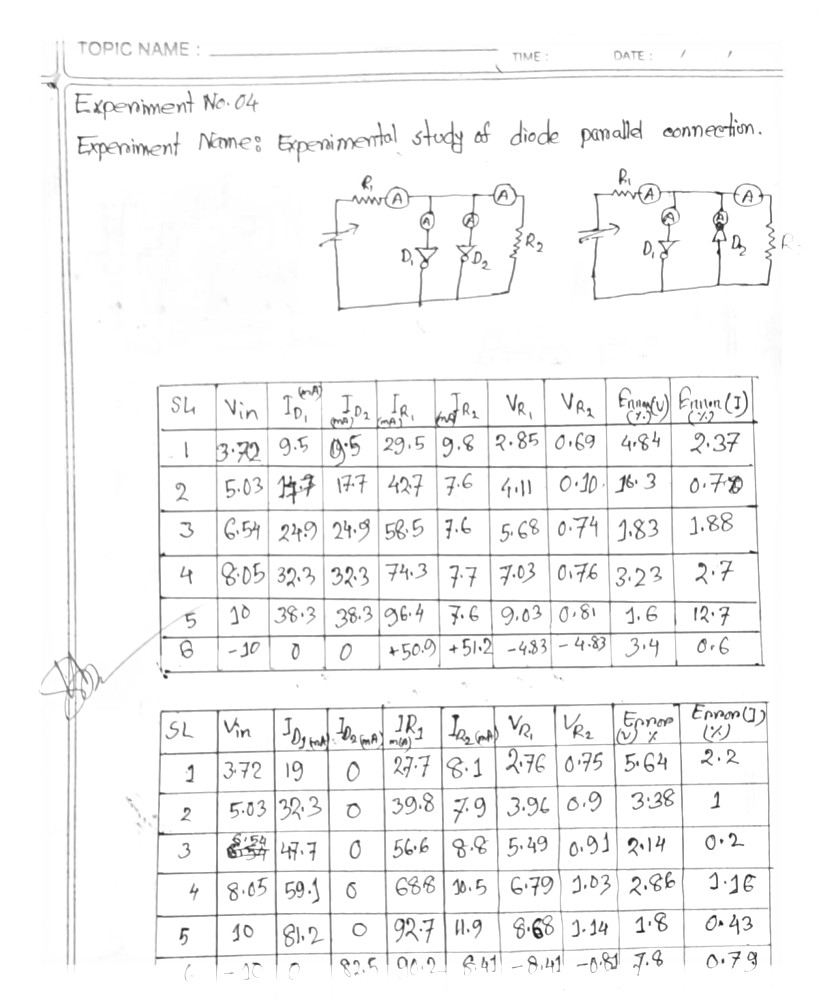
\includegraphics[scale=0.6]{src/exp03/r2.jpg}

    \caption{}
\end{figure}